\documentclass[1p]{elsarticle_modified}
%\bibliographystyle{elsarticle-num}

%\usepackage[colorlinks]{hyperref}
%\usepackage{abbrmath_seonhwa} %\Abb, \Ascr, \Acal ,\Abf, \Afrak
\usepackage{amsfonts}
\usepackage{amssymb}
\usepackage{amsmath}
\usepackage{amsthm}
\usepackage{scalefnt}
\usepackage{amsbsy}
\usepackage{kotex}
\usepackage{caption}
\usepackage{subfig}
\usepackage{color}
\usepackage{graphicx}
\usepackage{xcolor} %% white, black, red, green, blue, cyan, magenta, yellow
\usepackage{float}
\usepackage{setspace}
\usepackage{hyperref}

\usepackage{tikz}
\usetikzlibrary{arrows}

\usepackage{multirow}
\usepackage{array} % fixed length table
\usepackage{hhline}

%%%%%%%%%%%%%%%%%%%%%
\makeatletter
\renewcommand*\env@matrix[1][\arraystretch]{%
	\edef\arraystretch{#1}%
	\hskip -\arraycolsep
	\let\@ifnextchar\new@ifnextchar
	\array{*\c@MaxMatrixCols c}}
\makeatother %https://tex.stackexchange.com/questions/14071/how-can-i-increase-the-line-spacing-in-a-matrix
%%%%%%%%%%%%%%%

\usepackage[normalem]{ulem}

\newcommand{\msout}[1]{\ifmmode\text{\sout{\ensuremath{#1}}}\else\sout{#1}\fi}
%SOURCE: \msout is \stkout macro in https://tex.stackexchange.com/questions/20609/strikeout-in-math-mode

\newcommand{\cancel}[1]{
	\ifmmode
	{\color{red}\msout{#1}}
	\else
	{\color{red}\sout{#1}}
	\fi
}

\newcommand{\add}[1]{
	{\color{blue}\uwave{#1}}
}

\newcommand{\replace}[2]{
	\ifmmode
	{\color{red}\msout{#1}}{\color{blue}\uwave{#2}}
	\else
	{\color{red}\sout{#1}}{\color{blue}\uwave{#2}}
	\fi
}

\newcommand{\Sol}{\mathcal{S}} %segment
\newcommand{\D}{D} %diagram
\newcommand{\A}{\mathcal{A}} %arc


%%%%%%%%%%%%%%%%%%%%%%%%%%%%%5 test

\def\sl{\operatorname{\textup{SL}}(2,\Cbb)}
\def\psl{\operatorname{\textup{PSL}}(2,\Cbb)}
\def\quan{\mkern 1mu \triangleright \mkern 1mu}

\theoremstyle{definition}
\newtheorem{thm}{Theorem}[section]
\newtheorem{prop}[thm]{Proposition}
\newtheorem{lem}[thm]{Lemma}
\newtheorem{ques}[thm]{Question}
\newtheorem{cor}[thm]{Corollary}
\newtheorem{defn}[thm]{Definition}
\newtheorem{exam}[thm]{Example}
\newtheorem{rmk}[thm]{Remark}
\newtheorem{alg}[thm]{Algorithm}

\newcommand{\I}{\sqrt{-1}}
\begin{document}

%\begin{frontmatter}
%
%\title{Boundary parabolic representations of knots up to 8 crossings}
%
%%% Group authors per affiliation:
%\author{Yunhi Cho} 
%\address{Department of Mathematics, University of Seoul, Seoul, Korea}
%\ead{yhcho@uos.ac.kr}
%
%
%\author{Seonhwa Kim} %\fnref{s_kim}}
%\address{Center for Geometry and Physics, Institute for Basic Science, Pohang, 37673, Korea}
%\ead{ryeona17@ibs.re.kr}
%
%\author{Hyuk Kim}
%\address{Department of Mathematical Sciences, Seoul National University, Seoul 08826, Korea}
%\ead{hyukkim@snu.ac.kr}
%
%\author{Seokbeom Yoon}
%\address{Department of Mathematical Sciences, Seoul National University, Seoul, 08826,  Korea}
%\ead{sbyoon15@snu.ac.kr}
%
%\begin{abstract}
%We find all boundary parabolic representation of knots up to 8 crossings.
%
%\end{abstract}
%\begin{keyword}
%    \MSC[2010] 57M25 
%\end{keyword}
%
%\end{frontmatter}

%\linenumbers
%\tableofcontents
%
\newcommand\colored[1]{\textcolor{white}{\rule[-0.35ex]{0.8em}{1.4ex}}\kern-0.8em\color{red} #1}%
%\newcommand\colored[1]{\textcolor{white}{ #1}\kern-2.17ex	\textcolor{white}{ #1}\kern-1.81ex	\textcolor{white}{ #1}\kern-2.15ex\color{red}#1	}

{\Large $\underline{11a_{209}~(K11a_{209})}$}

\setlength{\tabcolsep}{10pt}
\renewcommand{\arraystretch}{1.6}
\vspace{1cm}\begin{tabular}{m{100pt}>{\centering\arraybackslash}m{274pt}}
\multirow{5}{120pt}{
	\centering
	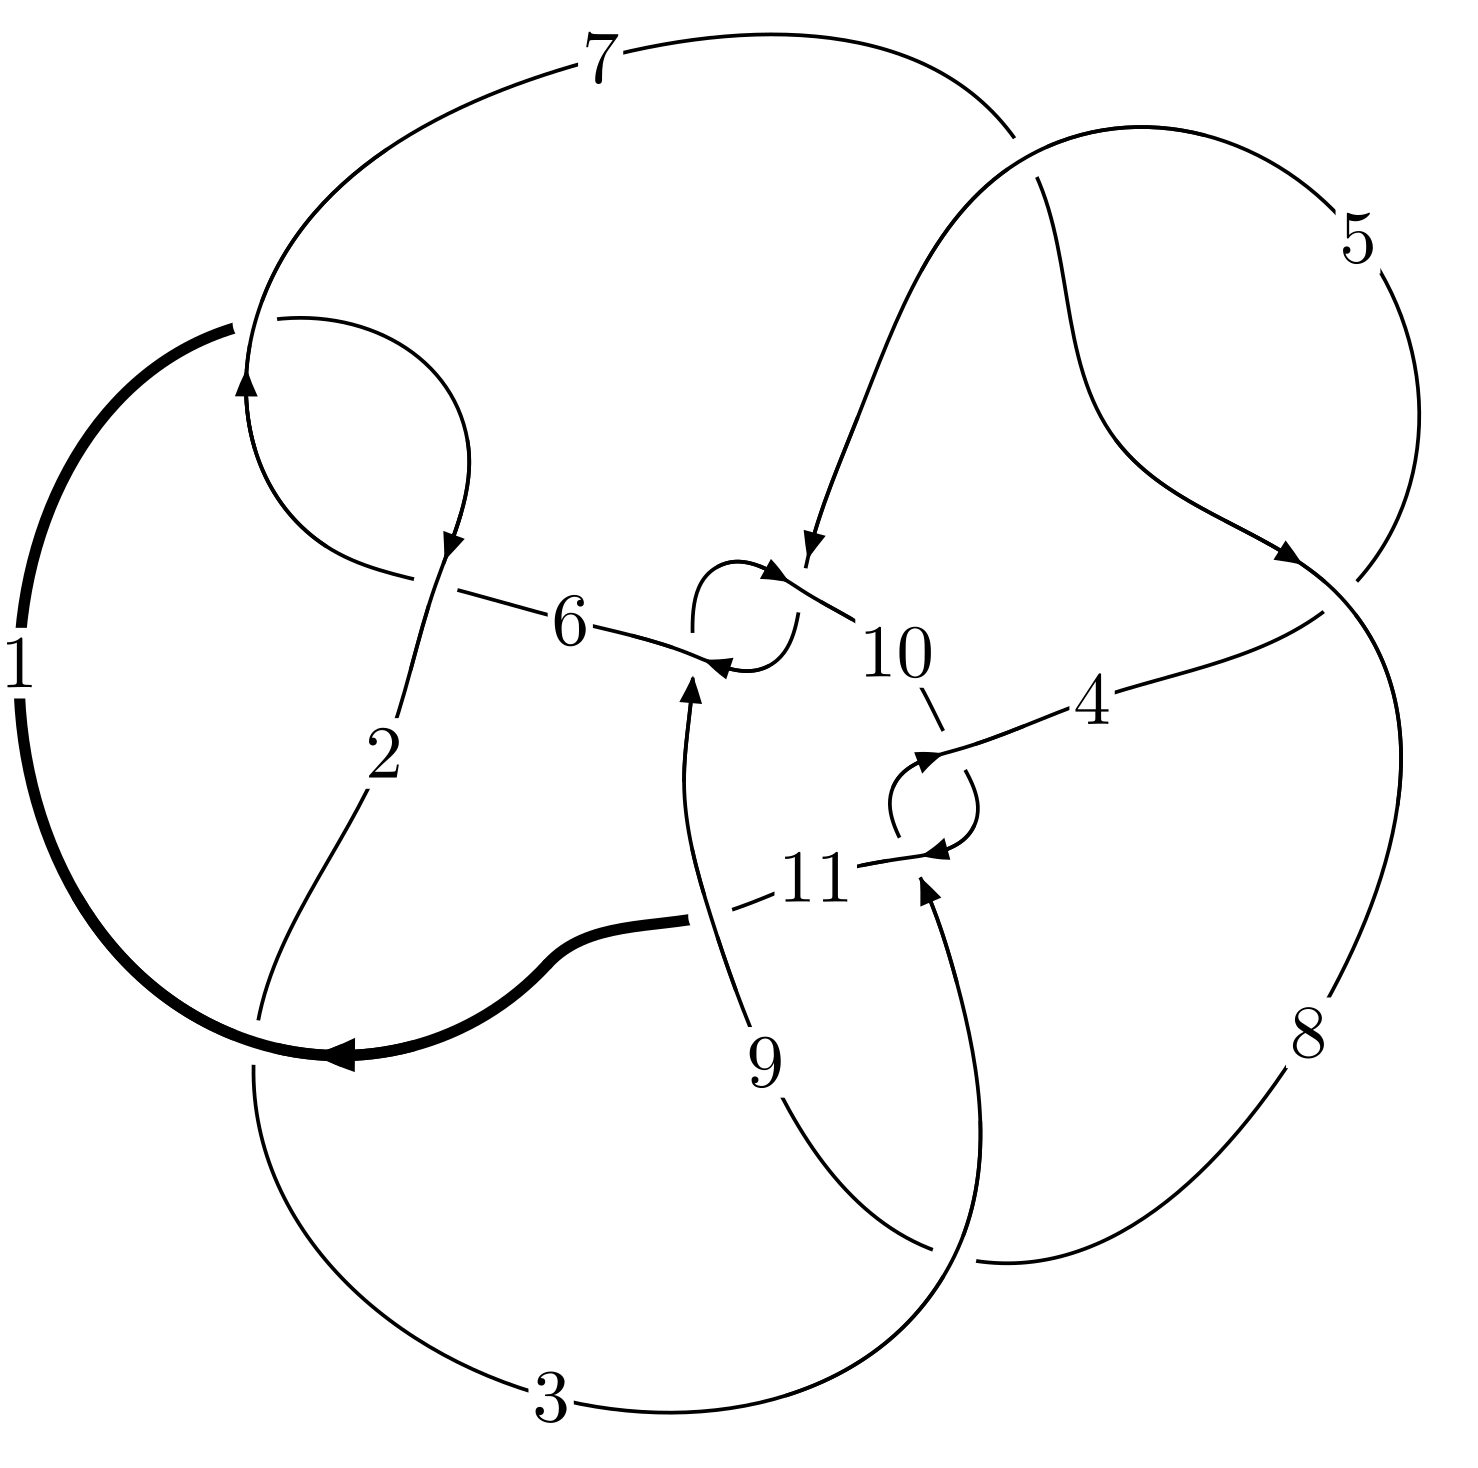
\includegraphics[width=112pt]{../../../GIT/diagram.site/Diagrams/png/458_11a_209.png}\\
\ \ \ A knot diagram\footnotemark}&
\allowdisplaybreaks
\textbf{Linearized knot diagam} \\
\cline{2-2}
 &
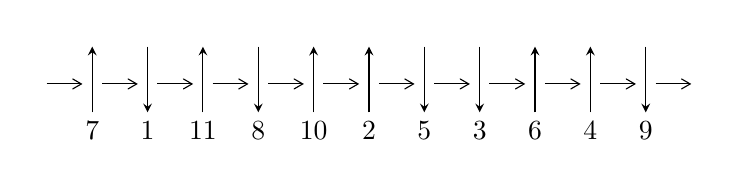
\begin{tikzpicture}[x=20pt, y=17pt]
	% nodes
	\node (C0) at (0, 0) {};
	\node (C1) at (1, 0) {};
	\node (C1U) at (1, +1) {};
	\node (C1D) at (1, -1) {7};

	\node (C2) at (2, 0) {};
	\node (C2U) at (2, +1) {};
	\node (C2D) at (2, -1) {1};

	\node (C3) at (3, 0) {};
	\node (C3U) at (3, +1) {};
	\node (C3D) at (3, -1) {11};

	\node (C4) at (4, 0) {};
	\node (C4U) at (4, +1) {};
	\node (C4D) at (4, -1) {8};

	\node (C5) at (5, 0) {};
	\node (C5U) at (5, +1) {};
	\node (C5D) at (5, -1) {10};

	\node (C6) at (6, 0) {};
	\node (C6U) at (6, +1) {};
	\node (C6D) at (6, -1) {2};

	\node (C7) at (7, 0) {};
	\node (C7U) at (7, +1) {};
	\node (C7D) at (7, -1) {5};

	\node (C8) at (8, 0) {};
	\node (C8U) at (8, +1) {};
	\node (C8D) at (8, -1) {3};

	\node (C9) at (9, 0) {};
	\node (C9U) at (9, +1) {};
	\node (C9D) at (9, -1) {6};

	\node (C10) at (10, 0) {};
	\node (C10U) at (10, +1) {};
	\node (C10D) at (10, -1) {4};

	\node (C11) at (11, 0) {};
	\node (C11U) at (11, +1) {};
	\node (C11D) at (11, -1) {9};
	\node (C12) at (12, 0) {};

	% arrows
	\draw[->,>={angle 60}]
	(C0) edge (C1) (C1) edge (C2) (C2) edge (C3) (C3) edge (C4) (C4) edge (C5) (C5) edge (C6) (C6) edge (C7) (C7) edge (C8) (C8) edge (C9) (C9) edge (C10) (C10) edge (C11) (C11) edge (C12) ;	\draw[->,>=stealth]
	(C1D) edge (C1U) (C2U) edge (C2D) (C3D) edge (C3U) (C4U) edge (C4D) (C5D) edge (C5U) (C6D) edge (C6U) (C7U) edge (C7D) (C8U) edge (C8D) (C9D) edge (C9U) (C10D) edge (C10U) (C11U) edge (C11D) ;
	\end{tikzpicture} \\
\hhline{~~} \\& 
\textbf{Solving Sequence} \\ \cline{2-2} 
 &
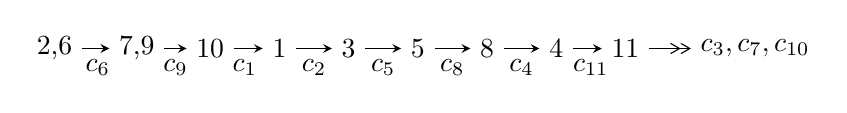
\begin{tikzpicture}[x=25pt, y=7pt]
	% node
	\node (A0) at (-1/8, 0) {2,6};
	\node (A1) at (17/16, 0) {7,9};
	\node (A2) at (17/8, 0) {10};
	\node (A3) at (25/8, 0) {1};
	\node (A4) at (33/8, 0) {3};
	\node (A5) at (41/8, 0) {5};
	\node (A6) at (49/8, 0) {8};
	\node (A7) at (57/8, 0) {4};
	\node (A8) at (65/8, 0) {11};
	\node (C1) at (1/2, -1) {$c_{6}$};
	\node (C2) at (13/8, -1) {$c_{9}$};
	\node (C3) at (21/8, -1) {$c_{1}$};
	\node (C4) at (29/8, -1) {$c_{2}$};
	\node (C5) at (37/8, -1) {$c_{5}$};
	\node (C6) at (45/8, -1) {$c_{8}$};
	\node (C7) at (53/8, -1) {$c_{4}$};
	\node (C8) at (61/8, -1) {$c_{11}$};
	\node (A9) at (10, 0) {$c_{3},c_{7},c_{10}$};

	% edge
	\draw[->,>=stealth]	
	(A0) edge (A1) (A1) edge (A2) (A2) edge (A3) (A3) edge (A4) (A4) edge (A5) (A5) edge (A6) (A6) edge (A7) (A7) edge (A8) ;
	\draw[->>,>={angle 60}]	
	(A8) edge (A9);
\end{tikzpicture} \\ 

\end{tabular} \\

\footnotetext{
The image of knot diagram is generated by the software ``\textbf{Draw programme}" developed by Andrew Bartholomew(\url{http://www.layer8.co.uk/maths/draw/index.htm\#Running-draw}), where we modified some parts for our purpose(\url{https://github.com/CATsTAILs/LinksPainter}).
}\phantom \\ \newline 
\centering \textbf{Ideals for irreducible components\footnotemark of $X_{\text{par}}$} 
 
\begin{align*}
I^u_{1}&=\langle 
-6.30788\times10^{126} u^{85}-9.55625\times10^{125} u^{84}+\cdots+9.00015\times10^{126} b+6.05580\times10^{127},\\
\phantom{I^u_{1}}&\phantom{= \langle  }-2.03979\times10^{128} u^{85}-2.07030\times10^{128} u^{84}+\cdots+2.07003\times10^{128} a-3.57647\times10^{129},\\
\phantom{I^u_{1}}&\phantom{= \langle  }u^{86}+u^{85}+\cdots+22 u+23\rangle \\
I^u_{2}&=\langle 
-2 u^{14}-7 u^{12}+2 u^{11}-16 u^{10}+9 u^9-23 u^8+15 u^7-26 u^6+17 u^5-22 u^4+10 u^3-11 u^2+b+3 u-2,\\
\phantom{I^u_{2}}&\phantom{= \langle  }u^{14}+u^{13}+4 u^{12}+2 u^{11}+8 u^{10}+u^9+9 u^8-2 u^7+9 u^6-2 u^5+7 u^4+4 u^2+a+u-1,\\
\phantom{I^u_{2}}&\phantom{= \langle  }u^{16}+4 u^{14}- u^{13}+10 u^{12}-5 u^{11}+16 u^{10}-10 u^9+20 u^8-13 u^7+19 u^6-10 u^5+13 u^4-5 u^3+5 u^2- u+1\rangle \\
\\
\end{align*}
\raggedright * 2 irreducible components of $\dim_{\mathbb{C}}=0$, with total 102 representations.\\
\footnotetext{All coefficients of polynomials are rational numbers. But the coefficients are sometimes approximated in decimal forms when there is not enough margin.}
\newpage
\renewcommand{\arraystretch}{1}
\centering \section*{I. $I^u_{1}= \langle -6.31\times10^{126} u^{85}-9.56\times10^{125} u^{84}+\cdots+9.00\times10^{126} b+6.06\times10^{127},\;-2.04\times10^{128} u^{85}-2.07\times10^{128} u^{84}+\cdots+2.07\times10^{128} a-3.58\times10^{129},\;u^{86}+u^{85}+\cdots+22 u+23 \rangle$}
\flushleft \textbf{(i) Arc colorings}\\
\begin{tabular}{m{7pt} m{180pt} m{7pt} m{180pt} }
\flushright $a_{2}=$&$\begin{pmatrix}0\\u\end{pmatrix}$ \\
\flushright $a_{6}=$&$\begin{pmatrix}1\\0\end{pmatrix}$ \\
\flushright $a_{7}=$&$\begin{pmatrix}1\\- u^2\end{pmatrix}$ \\
\flushright $a_{9}=$&$\begin{pmatrix}0.985388 u^{85}+1.00013 u^{84}+\cdots+21.7854 u+17.2774\\0.700864 u^{85}+0.106179 u^{84}+\cdots+14.6782 u-6.72856\end{pmatrix}$ \\
\flushright $a_{10}=$&$\begin{pmatrix}1.68625 u^{85}+1.10631 u^{84}+\cdots+36.4636 u+10.5488\\0.700864 u^{85}+0.106179 u^{84}+\cdots+14.6782 u-6.72856\end{pmatrix}$ \\
\flushright $a_{1}=$&$\begin{pmatrix}- u\\u^3+u\end{pmatrix}$ \\
\flushright $a_{3}=$&$\begin{pmatrix}- u^3\\u^5+u^3+u\end{pmatrix}$ \\
\flushright $a_{5}=$&$\begin{pmatrix}0.179613 u^{85}+0.843358 u^{84}+\cdots-1.56088 u+10.9518\\0.440284 u^{85}+0.983845 u^{84}+\cdots+15.9276 u+22.9163\end{pmatrix}$ \\
\flushright $a_{8}=$&$\begin{pmatrix}1.68776 u^{85}+1.23127 u^{84}+\cdots+40.7914 u+14.3817\\0.860452 u^{85}+0.154872 u^{84}+\cdots+20.0925 u-6.09132\end{pmatrix}$ \\
\flushright $a_{4}=$&$\begin{pmatrix}1.13364 u^{85}+1.30317 u^{84}+\cdots+25.1297 u+21.3228\\0.585302 u^{85}+0.634965 u^{84}+\cdots+18.0615 u+12.8964\end{pmatrix}$ \\
\flushright $a_{11}=$&$\begin{pmatrix}-0.151976 u^{85}-0.909808 u^{84}+\cdots-7.21246 u-14.7505\\0.0869857 u^{85}-0.573926 u^{84}+\cdots-0.0631483 u-8.62579\end{pmatrix}$\\ \flushright $a_{11}=$&$\begin{pmatrix}-0.151976 u^{85}-0.909808 u^{84}+\cdots-7.21246 u-14.7505\\0.0869857 u^{85}-0.573926 u^{84}+\cdots-0.0631483 u-8.62579\end{pmatrix}$\\&\end{tabular}
\flushleft \textbf{(ii) Obstruction class $= -1$}\\~\\
\flushleft \textbf{(iii) Cusp Shapes $= -2.93906 u^{85}-1.80148 u^{84}+\cdots-94.0864 u-29.1762$}\\~\\
\newpage\renewcommand{\arraystretch}{1}
\flushleft \textbf{(iv) u-Polynomials at the component}\newline \\
\begin{tabular}{m{50pt}|m{274pt}}
Crossings & \hspace{64pt}u-Polynomials at each crossing \\
\hline $$\begin{aligned}c_{1},c_{6}\end{aligned}$$&$\begin{aligned}
&u^{86}+u^{85}+\cdots+22 u+23
\end{aligned}$\\
\hline $$\begin{aligned}c_{2}\end{aligned}$$&$\begin{aligned}
&u^{86}+37 u^{85}+\cdots+8624 u+529
\end{aligned}$\\
\hline $$\begin{aligned}c_{3},c_{10}\end{aligned}$$&$\begin{aligned}
&u^{86}+5 u^{85}+\cdots+228 u+34
\end{aligned}$\\
\hline $$\begin{aligned}c_{4},c_{7}\end{aligned}$$&$\begin{aligned}
&u^{86}-3 u^{85}+\cdots-3 u+1
\end{aligned}$\\
\hline $$\begin{aligned}c_{5},c_{9}\end{aligned}$$&$\begin{aligned}
&u^{86}- u^{85}+\cdots+977 u+253
\end{aligned}$\\
\hline $$\begin{aligned}c_{8}\end{aligned}$$&$\begin{aligned}
&u^{86}+u^{85}+\cdots-5 u+1
\end{aligned}$\\
\hline $$\begin{aligned}c_{11}\end{aligned}$$&$\begin{aligned}
&u^{86}-3 u^{85}+\cdots-453 u+83
\end{aligned}$\\
\hline
\end{tabular}\\~\\
\newpage\renewcommand{\arraystretch}{1}
\flushleft \textbf{(v) Riley Polynomials at the component}\newline \\
\begin{tabular}{m{50pt}|m{274pt}}
Crossings & \hspace{64pt}Riley Polynomials at each crossing \\
\hline $$\begin{aligned}c_{1},c_{6}\end{aligned}$$&$\begin{aligned}
&y^{86}+37 y^{85}+\cdots+8624 y+529
\end{aligned}$\\
\hline $$\begin{aligned}c_{2}\end{aligned}$$&$\begin{aligned}
&y^{86}+33 y^{85}+\cdots+1800508 y+279841
\end{aligned}$\\
\hline $$\begin{aligned}c_{3},c_{10}\end{aligned}$$&$\begin{aligned}
&y^{86}+61 y^{85}+\cdots+39068 y+1156
\end{aligned}$\\
\hline $$\begin{aligned}c_{4},c_{7}\end{aligned}$$&$\begin{aligned}
&y^{86}+51 y^{85}+\cdots+79 y+1
\end{aligned}$\\
\hline $$\begin{aligned}c_{5},c_{9}\end{aligned}$$&$\begin{aligned}
&y^{86}+57 y^{85}+\cdots+492125 y+64009
\end{aligned}$\\
\hline $$\begin{aligned}c_{8}\end{aligned}$$&$\begin{aligned}
&y^{86}+7 y^{85}+\cdots+89 y+1
\end{aligned}$\\
\hline $$\begin{aligned}c_{11}\end{aligned}$$&$\begin{aligned}
&y^{86}-15 y^{85}+\cdots-330041 y+6889
\end{aligned}$\\
\hline
\end{tabular}\\~\\
\newpage\flushleft \textbf{(vi) Complex Volumes and Cusp Shapes}
$$\begin{array}{c|c|c}  
\text{Solutions to }I^u_{1}& \I (\text{vol} + \sqrt{-1}CS) & \text{Cusp shape}\\
 \hline 
\begin{aligned}
u &= -0.440608 + 0.882453 I \\
a &= -1.41549 + 0.11610 I \\
b &= -0.14456 - 2.08024 I\end{aligned}
 & -6.69565 - 1.80753 I & \phantom{-0.000000 } 0 \\ \hline\begin{aligned}
u &= -0.440608 - 0.882453 I \\
a &= -1.41549 - 0.11610 I \\
b &= -0.14456 + 2.08024 I\end{aligned}
 & -6.69565 + 1.80753 I & \phantom{-0.000000 } 0 \\ \hline\begin{aligned}
u &= \phantom{-}0.435411 + 0.874421 I \\
a &= \phantom{-}2.18520 - 0.30062 I \\
b &= -0.236877 - 0.859775 I\end{aligned}
 & -0.020421 + 1.232540 I & \phantom{-0.000000 } 0 \\ \hline\begin{aligned}
u &= \phantom{-}0.435411 - 0.874421 I \\
a &= \phantom{-}2.18520 + 0.30062 I \\
b &= -0.236877 + 0.859775 I\end{aligned}
 & -0.020421 - 1.232540 I & \phantom{-0.000000 } 0 \\ \hline\begin{aligned}
u &= -0.254148 + 0.997671 I \\
a &= -0.0121662 - 0.0653344 I \\
b &= \phantom{-}0.658248 + 0.624038 I\end{aligned}
 & -3.68445 - 0.23182 I & \phantom{-0.000000 } 0 \\ \hline\begin{aligned}
u &= -0.254148 - 0.997671 I \\
a &= -0.0121662 + 0.0653344 I \\
b &= \phantom{-}0.658248 - 0.624038 I\end{aligned}
 & -3.68445 + 0.23182 I & \phantom{-0.000000 } 0 \\ \hline\begin{aligned}
u &= \phantom{-}0.472137 + 0.915188 I \\
a &= -0.650907 + 0.686202 I \\
b &= \phantom{-}0.557676 - 0.372423 I\end{aligned}
 & -0.27091 + 2.38443 I & \phantom{-0.000000 } 0 \\ \hline\begin{aligned}
u &= \phantom{-}0.472137 - 0.915188 I \\
a &= -0.650907 - 0.686202 I \\
b &= \phantom{-}0.557676 + 0.372423 I\end{aligned}
 & -0.27091 - 2.38443 I & \phantom{-0.000000 } 0 \\ \hline\begin{aligned}
u &= \phantom{-}0.819335 + 0.516743 I \\
a &= \phantom{-}0.735754 - 1.133700 I \\
b &= -0.303943 + 1.157700 I\end{aligned}
 & -4.27251 - 4.47107 I & \phantom{-0.000000 } 0 \\ \hline\begin{aligned}
u &= \phantom{-}0.819335 - 0.516743 I \\
a &= \phantom{-}0.735754 + 1.133700 I \\
b &= -0.303943 - 1.157700 I\end{aligned}
 & -4.27251 + 4.47107 I & \phantom{-0.000000 } 0\\
 \hline 
 \end{array}$$\newpage$$\begin{array}{c|c|c}  
\text{Solutions to }I^u_{1}& \I (\text{vol} + \sqrt{-1}CS) & \text{Cusp shape}\\
 \hline 
\begin{aligned}
u &= -0.799498 + 0.671496 I \\
a &= -1.082950 - 0.476132 I \\
b &= \phantom{-}0.862405 - 0.332801 I\end{aligned}
 & \phantom{-}6.03113 - 0.23797 I & \phantom{-0.000000 } 0 \\ \hline\begin{aligned}
u &= -0.799498 - 0.671496 I \\
a &= -1.082950 + 0.476132 I \\
b &= \phantom{-}0.862405 + 0.332801 I\end{aligned}
 & \phantom{-}6.03113 + 0.23797 I & \phantom{-0.000000 } 0 \\ \hline\begin{aligned}
u &= \phantom{-}0.519186 + 0.913358 I \\
a &= -1.30951 + 1.25452 I \\
b &= \phantom{-}0.235203 + 1.254150 I\end{aligned}
 & \phantom{-}0.55328 + 3.31179 I & \phantom{-0.000000 } 0 \\ \hline\begin{aligned}
u &= \phantom{-}0.519186 - 0.913358 I \\
a &= -1.30951 - 1.25452 I \\
b &= \phantom{-}0.235203 - 1.254150 I\end{aligned}
 & \phantom{-}0.55328 - 3.31179 I & \phantom{-0.000000 } 0 \\ \hline\begin{aligned}
u &= \phantom{-}0.498753 + 0.796047 I \\
a &= \phantom{-}0.520912 + 0.215764 I \\
b &= -0.477711 + 1.141280 I\end{aligned}
 & \phantom{-}0.958565 + 0.837035 I & \phantom{-0.000000 } 0 \\ \hline\begin{aligned}
u &= \phantom{-}0.498753 - 0.796047 I \\
a &= \phantom{-}0.520912 - 0.215764 I \\
b &= -0.477711 - 1.141280 I\end{aligned}
 & \phantom{-}0.958565 - 0.837035 I & \phantom{-0.000000 } 0 \\ \hline\begin{aligned}
u &= -0.957226 + 0.470426 I \\
a &= -0.694272 - 0.926525 I \\
b &= \phantom{-}0.65505 + 1.27900 I\end{aligned}
 & -0.73034 + 11.32340 I & \phantom{-0.000000 } 0 \\ \hline\begin{aligned}
u &= -0.957226 - 0.470426 I \\
a &= -0.694272 + 0.926525 I \\
b &= \phantom{-}0.65505 - 1.27900 I\end{aligned}
 & -0.73034 - 11.32340 I & \phantom{-0.000000 } 0 \\ \hline\begin{aligned}
u &= \phantom{-}0.718222 + 0.590569 I \\
a &= -1.66020 + 0.78424 I \\
b &= \phantom{-}1.230230 + 0.333871 I\end{aligned}
 & \phantom{-}2.36607 - 4.79257 I & \phantom{-0.000000 } 0 \\ \hline\begin{aligned}
u &= \phantom{-}0.718222 - 0.590569 I \\
a &= -1.66020 - 0.78424 I \\
b &= \phantom{-}1.230230 - 0.333871 I\end{aligned}
 & \phantom{-}2.36607 + 4.79257 I & \phantom{-0.000000 } 0\\
 \hline 
 \end{array}$$\newpage$$\begin{array}{c|c|c}  
\text{Solutions to }I^u_{1}& \I (\text{vol} + \sqrt{-1}CS) & \text{Cusp shape}\\
 \hline 
\begin{aligned}
u &= -0.363945 + 0.853778 I \\
a &= \phantom{-}2.39581 + 1.39052 I \\
b &= \phantom{-}0.058045 + 0.753718 I\end{aligned}
 & -1.69428 + 3.12126 I & \phantom{-0.000000 } 0 \\ \hline\begin{aligned}
u &= -0.363945 - 0.853778 I \\
a &= \phantom{-}2.39581 - 1.39052 I \\
b &= \phantom{-}0.058045 - 0.753718 I\end{aligned}
 & -1.69428 - 3.12126 I & \phantom{-0.000000 } 0 \\ \hline\begin{aligned}
u &= \phantom{-}0.678602 + 0.851107 I \\
a &= \phantom{-}1.348950 + 0.317447 I \\
b &= -0.704996 - 0.539942 I\end{aligned}
 & \phantom{-}1.82473 + 1.72939 I & \phantom{-0.000000 } 0 \\ \hline\begin{aligned}
u &= \phantom{-}0.678602 - 0.851107 I \\
a &= \phantom{-}1.348950 - 0.317447 I \\
b &= -0.704996 + 0.539942 I\end{aligned}
 & \phantom{-}1.82473 - 1.72939 I & \phantom{-0.000000 } 0 \\ \hline\begin{aligned}
u &= \phantom{-}1.002180 + 0.442960 I \\
a &= -0.459083 + 0.579423 I \\
b &= \phantom{-}0.526479 - 1.140670 I\end{aligned}
 & \phantom{-}3.53168 - 4.85270 I & \phantom{-0.000000 } 0 \\ \hline\begin{aligned}
u &= \phantom{-}1.002180 - 0.442960 I \\
a &= -0.459083 - 0.579423 I \\
b &= \phantom{-}0.526479 + 1.140670 I\end{aligned}
 & \phantom{-}3.53168 + 4.85270 I & \phantom{-0.000000 } 0 \\ \hline\begin{aligned}
u &= -0.574135 + 0.697745 I \\
a &= \phantom{-}1.295480 + 0.432521 I \\
b &= -0.593842 - 0.982625 I\end{aligned}
 & \phantom{-}0.55800 + 3.23439 I & \phantom{-0.000000 } 0 \\ \hline\begin{aligned}
u &= -0.574135 - 0.697745 I \\
a &= \phantom{-}1.295480 - 0.432521 I \\
b &= -0.593842 + 0.982625 I\end{aligned}
 & \phantom{-}0.55800 - 3.23439 I & \phantom{-0.000000 } 0 \\ \hline\begin{aligned}
u &= -0.301901 + 1.060790 I \\
a &= \phantom{-}0.243556 + 0.478235 I \\
b &= \phantom{-}0.333285 + 0.966852 I\end{aligned}
 & -3.68916 - 0.50545 I & \phantom{-0.000000 } 0 \\ \hline\begin{aligned}
u &= -0.301901 - 1.060790 I \\
a &= \phantom{-}0.243556 - 0.478235 I \\
b &= \phantom{-}0.333285 - 0.966852 I\end{aligned}
 & -3.68916 + 0.50545 I & \phantom{-0.000000 } 0\\
 \hline 
 \end{array}$$\newpage$$\begin{array}{c|c|c}  
\text{Solutions to }I^u_{1}& \I (\text{vol} + \sqrt{-1}CS) & \text{Cusp shape}\\
 \hline 
\begin{aligned}
u &= -0.566298 + 0.952248 I \\
a &= -2.01719 - 1.25230 I \\
b &= \phantom{-}0.470639 - 1.102850 I\end{aligned}
 & -0.23044 - 7.80201 I & \phantom{-0.000000 } 0 \\ \hline\begin{aligned}
u &= -0.566298 - 0.952248 I \\
a &= -2.01719 + 1.25230 I \\
b &= \phantom{-}0.470639 + 1.102850 I\end{aligned}
 & -0.23044 + 7.80201 I & \phantom{-0.000000 } 0 \\ \hline\begin{aligned}
u &= -0.458991 + 1.014050 I \\
a &= -1.36992 - 0.61444 I \\
b &= \phantom{-}0.328045 + 0.090852 I\end{aligned}
 & -2.49113 - 6.25666 I & \phantom{-0.000000 } 0 \\ \hline\begin{aligned}
u &= -0.458991 - 1.014050 I \\
a &= -1.36992 + 0.61444 I \\
b &= \phantom{-}0.328045 - 0.090852 I\end{aligned}
 & -2.49113 + 6.25666 I & \phantom{-0.000000 } 0 \\ \hline\begin{aligned}
u &= -0.535541 + 0.976845 I \\
a &= \phantom{-}1.84339 - 0.12152 I \\
b &= -0.49099 + 1.53261 I\end{aligned}
 & -5.79066 - 2.94337 I & \phantom{-0.000000 } 0 \\ \hline\begin{aligned}
u &= -0.535541 - 0.976845 I \\
a &= \phantom{-}1.84339 + 0.12152 I \\
b &= -0.49099 - 1.53261 I\end{aligned}
 & -5.79066 + 2.94337 I & \phantom{-0.000000 } 0 \\ \hline\begin{aligned}
u &= \phantom{-}0.155910 + 0.854062 I \\
a &= \phantom{-}0.610198 - 1.248350 I \\
b &= -1.094600 + 0.553981 I\end{aligned}
 & -2.07684 - 4.50458 I & -4.60378 + 5.16323 I \\ \hline\begin{aligned}
u &= \phantom{-}0.155910 - 0.854062 I \\
a &= \phantom{-}0.610198 + 1.248350 I \\
b &= -1.094600 - 0.553981 I\end{aligned}
 & -2.07684 + 4.50458 I & -4.60378 - 5.16323 I \\ \hline\begin{aligned}
u &= \phantom{-}0.727983 + 0.866986 I \\
a &= -0.295618 + 1.161150 I \\
b &= \phantom{-}0.552356 - 0.433486 I\end{aligned}
 & \phantom{-}1.80523 + 3.66895 I & \phantom{-0.000000 } 0 \\ \hline\begin{aligned}
u &= \phantom{-}0.727983 - 0.866986 I \\
a &= -0.295618 - 1.161150 I \\
b &= \phantom{-}0.552356 + 0.433486 I\end{aligned}
 & \phantom{-}1.80523 - 3.66895 I & \phantom{-0.000000 } 0\\
 \hline 
 \end{array}$$\newpage$$\begin{array}{c|c|c}  
\text{Solutions to }I^u_{1}& \I (\text{vol} + \sqrt{-1}CS) & \text{Cusp shape}\\
 \hline 
\begin{aligned}
u &= \phantom{-}0.037161 + 1.155380 I \\
a &= -0.290467 - 0.823431 I \\
b &= \phantom{-}0.16766 - 1.42237 I\end{aligned}
 & -10.06360 - 2.70380 I & \phantom{-0.000000 } 0 \\ \hline\begin{aligned}
u &= \phantom{-}0.037161 - 1.155380 I \\
a &= -0.290467 + 0.823431 I \\
b &= \phantom{-}0.16766 + 1.42237 I\end{aligned}
 & -10.06360 + 2.70380 I & \phantom{-0.000000 } 0 \\ \hline\begin{aligned}
u &= \phantom{-}0.356735 + 1.106460 I \\
a &= \phantom{-}0.771475 + 0.196566 I \\
b &= \phantom{-}0.51455 - 1.45263 I\end{aligned}
 & -4.90859 - 0.03496 I & \phantom{-0.000000 } 0 \\ \hline\begin{aligned}
u &= \phantom{-}0.356735 - 1.106460 I \\
a &= \phantom{-}0.771475 - 0.196566 I \\
b &= \phantom{-}0.51455 + 1.45263 I\end{aligned}
 & -4.90859 + 0.03496 I & \phantom{-0.000000 } 0 \\ \hline\begin{aligned}
u &= -0.784201 + 0.874304 I \\
a &= \phantom{-}0.646233 - 1.252980 I \\
b &= -0.075808 + 0.802027 I\end{aligned}
 & \phantom{-}3.13190 - 2.94290 I & \phantom{-0.000000 } 0 \\ \hline\begin{aligned}
u &= -0.784201 - 0.874304 I \\
a &= \phantom{-}0.646233 + 1.252980 I \\
b &= -0.075808 - 0.802027 I\end{aligned}
 & \phantom{-}3.13190 + 2.94290 I & \phantom{-0.000000 } 0 \\ \hline\begin{aligned}
u &= \phantom{-}0.471061 + 1.075990 I \\
a &= -1.75793 + 0.83086 I \\
b &= \phantom{-}0.99776 + 1.30307 I\end{aligned}
 & -4.20557 + 7.31255 I & \phantom{-0.000000 } 0 \\ \hline\begin{aligned}
u &= \phantom{-}0.471061 - 1.075990 I \\
a &= -1.75793 - 0.83086 I \\
b &= \phantom{-}0.99776 - 1.30307 I\end{aligned}
 & -4.20557 - 7.31255 I & \phantom{-0.000000 } 0 \\ \hline\begin{aligned}
u &= -0.651807 + 0.489532 I \\
a &= \phantom{-}0.39844 - 1.41823 I \\
b &= \phantom{-}0.197920 + 1.236210 I\end{aligned}
 & -4.44910 - 1.59822 I & -3.44505 + 3.04430 I \\ \hline\begin{aligned}
u &= -0.651807 - 0.489532 I \\
a &= \phantom{-}0.39844 + 1.41823 I \\
b &= \phantom{-}0.197920 - 1.236210 I\end{aligned}
 & -4.44910 + 1.59822 I & -3.44505 - 3.04430 I\\
 \hline 
 \end{array}$$\newpage$$\begin{array}{c|c|c}  
\text{Solutions to }I^u_{1}& \I (\text{vol} + \sqrt{-1}CS) & \text{Cusp shape}\\
 \hline 
\begin{aligned}
u &= \phantom{-}0.624334 + 1.022790 I \\
a &= \phantom{-}0.969124 - 0.965579 I \\
b &= -1.47236 + 0.18895 I\end{aligned}
 & \phantom{-}1.06511 + 9.94951 I & \phantom{-0.000000 } 0 \\ \hline\begin{aligned}
u &= \phantom{-}0.624334 - 1.022790 I \\
a &= \phantom{-}0.969124 + 0.965579 I \\
b &= -1.47236 - 0.18895 I\end{aligned}
 & \phantom{-}1.06511 - 9.94951 I & \phantom{-0.000000 } 0 \\ \hline\begin{aligned}
u &= -0.788393 + 0.093088 I \\
a &= \phantom{-}0.175436 + 0.306457 I \\
b &= \phantom{-}0.330111 + 0.644700 I\end{aligned}
 & \phantom{-}0.40272 - 2.72268 I & \phantom{-}2.86940 + 3.16788 I \\ \hline\begin{aligned}
u &= -0.788393 - 0.093088 I \\
a &= \phantom{-}0.175436 - 0.306457 I \\
b &= \phantom{-}0.330111 - 0.644700 I\end{aligned}
 & \phantom{-}0.40272 + 2.72268 I & \phantom{-}2.86940 - 3.16788 I \\ \hline\begin{aligned}
u &= -0.683162 + 0.995349 I \\
a &= \phantom{-}0.756961 + 0.517256 I \\
b &= -0.997716 - 0.121911 I\end{aligned}
 & \phantom{-}5.03331 - 5.32903 I & \phantom{-0.000000 } 0 \\ \hline\begin{aligned}
u &= -0.683162 - 0.995349 I \\
a &= \phantom{-}0.756961 - 0.517256 I \\
b &= -0.997716 + 0.121911 I\end{aligned}
 & \phantom{-}5.03331 + 5.32903 I & \phantom{-0.000000 } 0 \\ \hline\begin{aligned}
u &= -0.536132 + 1.087660 I \\
a &= -1.55660 - 0.83006 I \\
b &= \phantom{-}0.756634 - 0.727652 I\end{aligned}
 & -2.10386 - 6.56947 I & \phantom{-0.000000 } 0 \\ \hline\begin{aligned}
u &= -0.536132 - 1.087660 I \\
a &= -1.55660 + 0.83006 I \\
b &= \phantom{-}0.756634 + 0.727652 I\end{aligned}
 & -2.10386 + 6.56947 I & \phantom{-0.000000 } 0 \\ \hline\begin{aligned}
u &= -0.573481 + 1.085080 I \\
a &= -1.67333 - 0.55597 I \\
b &= \phantom{-}0.531502 - 0.970130 I\end{aligned}
 & -1.93850 - 6.65557 I & \phantom{-0.000000 } 0 \\ \hline\begin{aligned}
u &= -0.573481 - 1.085080 I \\
a &= -1.67333 + 0.55597 I \\
b &= \phantom{-}0.531502 + 0.970130 I\end{aligned}
 & -1.93850 + 6.65557 I & \phantom{-0.000000 } 0\\
 \hline 
 \end{array}$$\newpage$$\begin{array}{c|c|c}  
\text{Solutions to }I^u_{1}& \I (\text{vol} + \sqrt{-1}CS) & \text{Cusp shape}\\
 \hline 
\begin{aligned}
u &= \phantom{-}1.131390 + 0.532631 I \\
a &= -0.273567 - 0.463197 I \\
b &= \phantom{-}0.248035 + 0.937067 I\end{aligned}
 & -0.23931 + 5.38129 I & \phantom{-0.000000 } 0 \\ \hline\begin{aligned}
u &= \phantom{-}1.131390 - 0.532631 I \\
a &= -0.273567 + 0.463197 I \\
b &= \phantom{-}0.248035 - 0.937067 I\end{aligned}
 & -0.23931 - 5.38129 I & \phantom{-0.000000 } 0 \\ \hline\begin{aligned}
u &= \phantom{-}0.657555 + 1.085690 I \\
a &= -1.92694 + 0.01672 I \\
b &= \phantom{-}0.437325 + 1.219940 I\end{aligned}
 & -5.97898 + 10.01160 I & \phantom{-0.000000 } 0 \\ \hline\begin{aligned}
u &= \phantom{-}0.657555 - 1.085690 I \\
a &= -1.92694 - 0.01672 I \\
b &= \phantom{-}0.437325 - 1.219940 I\end{aligned}
 & -5.97898 - 10.01160 I & \phantom{-0.000000 } 0 \\ \hline\begin{aligned}
u &= -0.613434 + 0.381423 I \\
a &= \phantom{-}1.142460 + 0.688198 I \\
b &= -0.522004 - 0.772282 I\end{aligned}
 & \phantom{-}0.03093 + 1.91449 I & \phantom{-}1.42093 - 2.93716 I \\ \hline\begin{aligned}
u &= -0.613434 - 0.381423 I \\
a &= \phantom{-}1.142460 - 0.688198 I \\
b &= -0.522004 + 0.772282 I\end{aligned}
 & \phantom{-}0.03093 - 1.91449 I & \phantom{-}1.42093 + 2.93716 I \\ \hline\begin{aligned}
u &= -0.624780 + 0.343324 I \\
a &= \phantom{-}1.41145 + 0.48892 I \\
b &= -0.637437 - 0.540547 I\end{aligned}
 & \phantom{-}0.00762 + 1.99264 I & \phantom{-}2.82106 - 2.47705 I \\ \hline\begin{aligned}
u &= -0.624780 - 0.343324 I \\
a &= \phantom{-}1.41145 - 0.48892 I \\
b &= -0.637437 + 0.540547 I\end{aligned}
 & \phantom{-}0.00762 - 1.99264 I & \phantom{-}2.82106 + 2.47705 I \\ \hline\begin{aligned}
u &= \phantom{-}0.006838 + 1.320150 I \\
a &= -0.042358 - 0.568413 I \\
b &= -0.369980 - 1.292530 I\end{aligned}
 & -7.52252 + 8.52696 I & \phantom{-0.000000 } 0 \\ \hline\begin{aligned}
u &= \phantom{-}0.006838 - 1.320150 I \\
a &= -0.042358 + 0.568413 I \\
b &= -0.369980 + 1.292530 I\end{aligned}
 & -7.52252 - 8.52696 I & \phantom{-0.000000 } 0\\
 \hline 
 \end{array}$$\newpage$$\begin{array}{c|c|c}  
\text{Solutions to }I^u_{1}& \I (\text{vol} + \sqrt{-1}CS) & \text{Cusp shape}\\
 \hline 
\begin{aligned}
u &= -0.682783 + 1.148320 I \\
a &= \phantom{-}1.73833 + 0.37633 I \\
b &= -0.70195 + 1.39798 I\end{aligned}
 & -2.8205 - 17.3023 I & \phantom{-0.000000 } 0 \\ \hline\begin{aligned}
u &= -0.682783 - 1.148320 I \\
a &= \phantom{-}1.73833 - 0.37633 I \\
b &= -0.70195 - 1.39798 I\end{aligned}
 & -2.8205 + 17.3023 I & \phantom{-0.000000 } 0 \\ \hline\begin{aligned}
u &= \phantom{-}0.385965 + 0.524461 I \\
a &= \phantom{-}1.33463 + 0.54748 I \\
b &= -0.346668 - 0.264256 I\end{aligned}
 & \phantom{-}0.610346 + 1.128090 I & \phantom{-}4.76161 - 5.52253 I \\ \hline\begin{aligned}
u &= \phantom{-}0.385965 - 0.524461 I \\
a &= \phantom{-}1.33463 - 0.54748 I \\
b &= -0.346668 + 0.264256 I\end{aligned}
 & \phantom{-}0.610346 - 1.128090 I & \phantom{-}4.76161 + 5.52253 I \\ \hline\begin{aligned}
u &= \phantom{-}0.689193 + 1.161250 I \\
a &= \phantom{-}1.45571 - 0.42058 I \\
b &= -0.55690 - 1.30946 I\end{aligned}
 & \phantom{-}1.32319 + 10.94470 I & \phantom{-0.000000 } 0 \\ \hline\begin{aligned}
u &= \phantom{-}0.689193 - 1.161250 I \\
a &= \phantom{-}1.45571 + 0.42058 I \\
b &= -0.55690 + 1.30946 I\end{aligned}
 & \phantom{-}1.32319 - 10.94470 I & \phantom{-0.000000 } 0 \\ \hline\begin{aligned}
u &= -0.178929 + 1.357480 I \\
a &= \phantom{-}0.024553 + 0.644724 I \\
b &= -0.122682 + 1.122470 I\end{aligned}
 & -4.10884 - 1.64866 I & \phantom{-0.000000 } 0 \\ \hline\begin{aligned}
u &= -0.178929 - 1.357480 I \\
a &= \phantom{-}0.024553 - 0.644724 I \\
b &= -0.122682 - 1.122470 I\end{aligned}
 & -4.10884 + 1.64866 I & \phantom{-0.000000 } 0 \\ \hline\begin{aligned}
u &= \phantom{-}0.591175 + 0.049975 I \\
a &= \phantom{-}1.31039 - 1.38090 I \\
b &= -0.687577 + 1.119080 I\end{aligned}
 & -1.62551 - 3.43865 I & -0.96501 + 2.90877 I \\ \hline\begin{aligned}
u &= \phantom{-}0.591175 - 0.049975 I \\
a &= \phantom{-}1.31039 + 1.38090 I \\
b &= -0.687577 - 1.119080 I\end{aligned}
 & -1.62551 + 3.43865 I & -0.96501 - 2.90877 I\\
 \hline 
 \end{array}$$\newpage$$\begin{array}{c|c|c}  
\text{Solutions to }I^u_{1}& \I (\text{vol} + \sqrt{-1}CS) & \text{Cusp shape}\\
 \hline 
\begin{aligned}
u &= \phantom{-}0.145997 + 0.558877 I \\
a &= \phantom{-}1.02027 + 1.15455 I \\
b &= -0.467675 - 0.564857 I\end{aligned}
 & \phantom{-}0.40918 + 1.48015 I & \phantom{-}2.24000 - 5.97587 I \\ \hline\begin{aligned}
u &= \phantom{-}0.145997 - 0.558877 I \\
a &= \phantom{-}1.02027 - 1.15455 I \\
b &= -0.467675 + 0.564857 I\end{aligned}
 & \phantom{-}0.40918 - 1.48015 I & \phantom{-}2.24000 + 5.97587 I \\ \hline\begin{aligned}
u &= \phantom{-}0.62384 + 1.28071 I \\
a &= -0.820261 + 0.152739 I \\
b &= -0.005790 + 0.909994 I\end{aligned}
 & -3.04048 + 1.33044 I & \phantom{-0.000000 } 0 \\ \hline\begin{aligned}
u &= \phantom{-}0.62384 - 1.28071 I \\
a &= -0.820261 - 0.152739 I \\
b &= -0.005790 - 0.909994 I\end{aligned}
 & -3.04048 - 1.33044 I & \phantom{-0.000000 } 0 \\ \hline\begin{aligned}
u &= -0.87956 + 1.15875 I \\
a &= \phantom{-}0.821875 - 0.111111 I \\
b &= -0.137121 + 1.346990 I\end{aligned}
 & -4.20851 - 3.78318 I & \phantom{-0.000000 } 0 \\ \hline\begin{aligned}
u &= -0.87956 - 1.15875 I \\
a &= \phantom{-}0.821875 + 0.111111 I \\
b &= -0.137121 - 1.346990 I\end{aligned}
 & -4.20851 + 3.78318 I & \phantom{-0.000000 } 0\\
 \hline 
 \end{array}$$\newpage\newpage\renewcommand{\arraystretch}{1}
\centering \section*{II. $I^u_{2}= \langle -2 u^{14}-7 u^{12}+\cdots+b-2,\;u^{14}+u^{13}+\cdots+a-1,\;u^{16}+4 u^{14}+\cdots- u+1 \rangle$}
\flushleft \textbf{(i) Arc colorings}\\
\begin{tabular}{m{7pt} m{180pt} m{7pt} m{180pt} }
\flushright $a_{2}=$&$\begin{pmatrix}0\\u\end{pmatrix}$ \\
\flushright $a_{6}=$&$\begin{pmatrix}1\\0\end{pmatrix}$ \\
\flushright $a_{7}=$&$\begin{pmatrix}1\\- u^2\end{pmatrix}$ \\
\flushright $a_{9}=$&$\begin{pmatrix}- u^{14}- u^{13}+\cdots- u+1\\2 u^{14}+7 u^{12}+\cdots-3 u+2\end{pmatrix}$ \\
\flushright $a_{10}=$&$\begin{pmatrix}u^{14}- u^{13}+\cdots-4 u+3\\2 u^{14}+7 u^{12}+\cdots-3 u+2\end{pmatrix}$ \\
\flushright $a_{1}=$&$\begin{pmatrix}- u\\u^3+u\end{pmatrix}$ \\
\flushright $a_{3}=$&$\begin{pmatrix}- u^3\\u^5+u^3+u\end{pmatrix}$ \\
\flushright $a_{5}=$&$\begin{pmatrix}2 u^{14}- u^{13}+\cdots-5 u+4\\u^{15}- u^{14}+\cdots+u-1\end{pmatrix}$ \\
\flushright $a_{8}=$&$\begin{pmatrix}- u^{13}- u^{12}+\cdots- u+1\\2 u^{14}+7 u^{12}+\cdots-3 u+2\end{pmatrix}$ \\
\flushright $a_{4}=$&$\begin{pmatrix}u^{15}+u^{14}+\cdots+4 u-2\\u^{15}- u^{14}+\cdots+2 u-1\end{pmatrix}$ \\
\flushright $a_{11}=$&$\begin{pmatrix}u^{15}+4 u^{13}+\cdots+3 u+3\\u^{15}+4 u^{13}+\cdots- u^2+u\end{pmatrix}$\\ \flushright $a_{11}=$&$\begin{pmatrix}u^{15}+4 u^{13}+\cdots+3 u+3\\u^{15}+4 u^{13}+\cdots- u^2+u\end{pmatrix}$\\&\end{tabular}
\flushleft \textbf{(ii) Obstruction class $= 1$}\\~\\
\flushleft \textbf{(iii) Cusp Shapes $= u^{15}- u^{14}+4 u^{13}+2 u^{12}+12 u^{11}+7 u^{10}+16 u^9+17 u^8+5 u^7+17 u^6- u^5+20 u^4-6 u^3+18 u^2+5$}\\~\\
\newpage\renewcommand{\arraystretch}{1}
\flushleft \textbf{(iv) u-Polynomials at the component}\newline \\
\begin{tabular}{m{50pt}|m{274pt}}
Crossings & \hspace{64pt}u-Polynomials at each crossing \\
\hline $$\begin{aligned}c_{1}\end{aligned}$$&$\begin{aligned}
&u^{16}+4 u^{14}+\cdots+u+1
\end{aligned}$\\
\hline $$\begin{aligned}c_{2}\end{aligned}$$&$\begin{aligned}
&u^{16}+8 u^{15}+\cdots+9 u+1
\end{aligned}$\\
\hline $$\begin{aligned}c_{3}\end{aligned}$$&$\begin{aligned}
&u^{16}+8 u^{14}+\cdots+u+2
\end{aligned}$\\
\hline $$\begin{aligned}c_{4}\end{aligned}$$&$\begin{aligned}
&u^{16}-2 u^{15}+\cdots+8 u^2+1
\end{aligned}$\\
\hline $$\begin{aligned}c_{5}\end{aligned}$$&$\begin{aligned}
&u^{16}+8 u^{14}+\cdots+2 u+1
\end{aligned}$\\
\hline $$\begin{aligned}c_{6}\end{aligned}$$&$\begin{aligned}
&u^{16}+4 u^{14}+\cdots- u+1
\end{aligned}$\\
\hline $$\begin{aligned}c_{7}\end{aligned}$$&$\begin{aligned}
&u^{16}+2 u^{15}+\cdots+8 u^2+1
\end{aligned}$\\
\hline $$\begin{aligned}c_{8}\end{aligned}$$&$\begin{aligned}
&u^{16}+3 u^{14}+\cdots-4 u+1
\end{aligned}$\\
\hline $$\begin{aligned}c_{9}\end{aligned}$$&$\begin{aligned}
&u^{16}+8 u^{14}+\cdots-2 u+1
\end{aligned}$\\
\hline $$\begin{aligned}c_{10}\end{aligned}$$&$\begin{aligned}
&u^{16}+8 u^{14}+\cdots- u+2
\end{aligned}$\\
\hline $$\begin{aligned}c_{11}\end{aligned}$$&$\begin{aligned}
&u^{16}+6 u^{15}+\cdots+5 u^3+1
\end{aligned}$\\
\hline
\end{tabular}\\~\\
\newpage\renewcommand{\arraystretch}{1}
\flushleft \textbf{(v) Riley Polynomials at the component}\newline \\
\begin{tabular}{m{50pt}|m{274pt}}
Crossings & \hspace{64pt}Riley Polynomials at each crossing \\
\hline $$\begin{aligned}c_{1},c_{6}\end{aligned}$$&$\begin{aligned}
&y^{16}+8 y^{15}+\cdots+9 y+1
\end{aligned}$\\
\hline $$\begin{aligned}c_{2}\end{aligned}$$&$\begin{aligned}
&y^{16}+8 y^{15}+\cdots+y+1
\end{aligned}$\\
\hline $$\begin{aligned}c_{3},c_{10}\end{aligned}$$&$\begin{aligned}
&y^{16}+16 y^{15}+\cdots+39 y+4
\end{aligned}$\\
\hline $$\begin{aligned}c_{4},c_{7}\end{aligned}$$&$\begin{aligned}
&y^{16}+14 y^{15}+\cdots+16 y+1
\end{aligned}$\\
\hline $$\begin{aligned}c_{5},c_{9}\end{aligned}$$&$\begin{aligned}
&y^{16}+16 y^{15}+\cdots+14 y+1
\end{aligned}$\\
\hline $$\begin{aligned}c_{8}\end{aligned}$$&$\begin{aligned}
&y^{16}+6 y^{15}+\cdots-2 y+1
\end{aligned}$\\
\hline $$\begin{aligned}c_{11}\end{aligned}$$&$\begin{aligned}
&y^{16}-4 y^{15}+\cdots+30 y^2+1
\end{aligned}$\\
\hline
\end{tabular}\\~\\
\newpage\flushleft \textbf{(vi) Complex Volumes and Cusp Shapes}
$$\begin{array}{c|c|c}  
\text{Solutions to }I^u_{2}& \I (\text{vol} + \sqrt{-1}CS) & \text{Cusp shape}\\
 \hline 
\begin{aligned}
u &= -0.343340 + 0.903837 I \\
a &= \phantom{-}1.56676 - 0.12174 I \\
b &= \phantom{-}0.11176 + 1.95777 I\end{aligned}
 & -7.14694 - 1.43565 I & -10.40664 - 2.32978 I \\ \hline\begin{aligned}
u &= -0.343340 - 0.903837 I \\
a &= \phantom{-}1.56676 + 0.12174 I \\
b &= \phantom{-}0.11176 - 1.95777 I\end{aligned}
 & -7.14694 + 1.43565 I & -10.40664 + 2.32978 I \\ \hline\begin{aligned}
u &= \phantom{-}0.798443 + 0.511463 I \\
a &= -0.0414475 + 0.0829013 I \\
b &= -0.318907 - 0.710933 I\end{aligned}
 & \phantom{-}0.31683 + 4.82313 I & \phantom{-}2.45674 - 4.45720 I \\ \hline\begin{aligned}
u &= \phantom{-}0.798443 - 0.511463 I \\
a &= -0.0414475 - 0.0829013 I \\
b &= -0.318907 + 0.710933 I\end{aligned}
 & \phantom{-}0.31683 - 4.82313 I & \phantom{-}2.45674 + 4.45720 I \\ \hline\begin{aligned}
u &= -0.738361 + 0.873406 I \\
a &= \phantom{-}0.552854 - 1.253860 I \\
b &= -0.051627 + 0.529275 I\end{aligned}
 & \phantom{-}3.66939 - 2.80776 I & \phantom{-}10.64447 + 1.16069 I \\ \hline\begin{aligned}
u &= -0.738361 - 0.873406 I \\
a &= \phantom{-}0.552854 + 1.253860 I \\
b &= -0.051627 - 0.529275 I\end{aligned}
 & \phantom{-}3.66939 + 2.80776 I & \phantom{-}10.64447 - 1.16069 I \\ \hline\begin{aligned}
u &= \phantom{-}0.487072 + 1.055760 I \\
a &= -1.83617 + 1.15350 I \\
b &= \phantom{-}0.700331 + 0.823488 I\end{aligned}
 & -2.30232 + 7.54648 I & -2.14299 - 11.74045 I \\ \hline\begin{aligned}
u &= \phantom{-}0.487072 - 1.055760 I \\
a &= -1.83617 - 1.15350 I \\
b &= \phantom{-}0.700331 - 0.823488 I\end{aligned}
 & -2.30232 - 7.54648 I & -2.14299 + 11.74045 I \\ \hline\begin{aligned}
u &= \phantom{-}0.327557 + 1.160530 I \\
a &= \phantom{-}0.563947 - 0.360432 I \\
b &= \phantom{-}0.311651 - 1.038780 I\end{aligned}
 & -2.86838 - 0.11828 I & -0.88069 + 2.46501 I \\ \hline\begin{aligned}
u &= \phantom{-}0.327557 - 1.160530 I \\
a &= \phantom{-}0.563947 + 0.360432 I \\
b &= \phantom{-}0.311651 + 1.038780 I\end{aligned}
 & -2.86838 + 0.11828 I & -0.88069 - 2.46501 I\\
 \hline 
 \end{array}$$\newpage$$\begin{array}{c|c|c}  
\text{Solutions to }I^u_{2}& \I (\text{vol} + \sqrt{-1}CS) & \text{Cusp shape}\\
 \hline 
\begin{aligned}
u &= \phantom{-}0.394909 + 0.626627 I \\
a &= \phantom{-}2.17510 - 1.35355 I \\
b &= -0.606467 + 0.609910 I\end{aligned}
 & -0.74107 - 3.74159 I & \phantom{-}1.01930 + 5.15973 I \\ \hline\begin{aligned}
u &= \phantom{-}0.394909 - 0.626627 I \\
a &= \phantom{-}2.17510 + 1.35355 I \\
b &= -0.606467 - 0.609910 I\end{aligned}
 & -0.74107 + 3.74159 I & \phantom{-}1.01930 - 5.15973 I \\ \hline\begin{aligned}
u &= -0.158611 + 0.649341 I \\
a &= \phantom{-}1.97289 - 0.31397 I \\
b &= -0.371932 - 0.795508 I\end{aligned}
 & \phantom{-}0.080629 + 0.400598 I & -1.246602 - 0.185548 I \\ \hline\begin{aligned}
u &= -0.158611 - 0.649341 I \\
a &= \phantom{-}1.97289 + 0.31397 I \\
b &= -0.371932 + 0.795508 I\end{aligned}
 & \phantom{-}0.080629 - 0.400598 I & -1.246602 + 0.185548 I \\ \hline\begin{aligned}
u &= -0.767670 + 1.139480 I \\
a &= -0.953934 + 0.004192 I \\
b &= \phantom{-}0.225194 - 1.371430 I\end{aligned}
 & -4.16761 - 3.51464 I & -0.94360 - 6.61638 I \\ \hline\begin{aligned}
u &= -0.767670 - 1.139480 I \\
a &= -0.953934 - 0.004192 I \\
b &= \phantom{-}0.225194 + 1.371430 I\end{aligned}
 & -4.16761 + 3.51464 I & -0.94360 + 6.61638 I\\
 \hline 
 \end{array}$$\newpage
\newpage\renewcommand{\arraystretch}{1}
\centering \section*{ III. u-Polynomials}
\begin{tabular}{m{50pt}|m{274pt}}
Crossings & \hspace{64pt}u-Polynomials at each crossing \\
\hline $$\begin{aligned}c_{1}\end{aligned}$$&$\begin{aligned}
&(u^{16}+4 u^{14}+\cdots+u+1)(u^{86}+u^{85}+\cdots+22 u+23)
\end{aligned}$\\
\hline $$\begin{aligned}c_{2}\end{aligned}$$&$\begin{aligned}
&(u^{16}+8 u^{15}+\cdots+9 u+1)(u^{86}+37 u^{85}+\cdots+8624 u+529)
\end{aligned}$\\
\hline $$\begin{aligned}c_{3}\end{aligned}$$&$\begin{aligned}
&(u^{16}+8 u^{14}+\cdots+u+2)(u^{86}+5 u^{85}+\cdots+228 u+34)
\end{aligned}$\\
\hline $$\begin{aligned}c_{4}\end{aligned}$$&$\begin{aligned}
&(u^{16}-2 u^{15}+\cdots+8 u^2+1)(u^{86}-3 u^{85}+\cdots-3 u+1)
\end{aligned}$\\
\hline $$\begin{aligned}c_{5}\end{aligned}$$&$\begin{aligned}
&(u^{16}+8 u^{14}+\cdots+2 u+1)(u^{86}- u^{85}+\cdots+977 u+253)
\end{aligned}$\\
\hline $$\begin{aligned}c_{6}\end{aligned}$$&$\begin{aligned}
&(u^{16}+4 u^{14}+\cdots- u+1)(u^{86}+u^{85}+\cdots+22 u+23)
\end{aligned}$\\
\hline $$\begin{aligned}c_{7}\end{aligned}$$&$\begin{aligned}
&(u^{16}+2 u^{15}+\cdots+8 u^2+1)(u^{86}-3 u^{85}+\cdots-3 u+1)
\end{aligned}$\\
\hline $$\begin{aligned}c_{8}\end{aligned}$$&$\begin{aligned}
&(u^{16}+3 u^{14}+\cdots-4 u+1)(u^{86}+u^{85}+\cdots-5 u+1)
\end{aligned}$\\
\hline $$\begin{aligned}c_{9}\end{aligned}$$&$\begin{aligned}
&(u^{16}+8 u^{14}+\cdots-2 u+1)(u^{86}- u^{85}+\cdots+977 u+253)
\end{aligned}$\\
\hline $$\begin{aligned}c_{10}\end{aligned}$$&$\begin{aligned}
&(u^{16}+8 u^{14}+\cdots- u+2)(u^{86}+5 u^{85}+\cdots+228 u+34)
\end{aligned}$\\
\hline $$\begin{aligned}c_{11}\end{aligned}$$&$\begin{aligned}
&(u^{16}+6 u^{15}+\cdots+5 u^3+1)(u^{86}-3 u^{85}+\cdots-453 u+83)
\end{aligned}$\\
\hline
\end{tabular}\newpage\renewcommand{\arraystretch}{1}
\centering \section*{ IV. Riley Polynomials}
\begin{tabular}{m{50pt}|m{274pt}}
Crossings & \hspace{64pt}Riley Polynomials at each crossing \\
\hline $$\begin{aligned}c_{1},c_{6}\end{aligned}$$&$\begin{aligned}
&(y^{16}+8 y^{15}+\cdots+9 y+1)(y^{86}+37 y^{85}+\cdots+8624 y+529)
\end{aligned}$\\
\hline $$\begin{aligned}c_{2}\end{aligned}$$&$\begin{aligned}
&(y^{16}+8 y^{15}+\cdots+y+1)(y^{86}+33 y^{85}+\cdots+1800508 y+279841)
\end{aligned}$\\
\hline $$\begin{aligned}c_{3},c_{10}\end{aligned}$$&$\begin{aligned}
&(y^{16}+16 y^{15}+\cdots+39 y+4)(y^{86}+61 y^{85}+\cdots+39068 y+1156)
\end{aligned}$\\
\hline $$\begin{aligned}c_{4},c_{7}\end{aligned}$$&$\begin{aligned}
&(y^{16}+14 y^{15}+\cdots+16 y+1)(y^{86}+51 y^{85}+\cdots+79 y+1)
\end{aligned}$\\
\hline $$\begin{aligned}c_{5},c_{9}\end{aligned}$$&$\begin{aligned}
&(y^{16}+16 y^{15}+\cdots+14 y+1)(y^{86}+57 y^{85}+\cdots+492125 y+64009)
\end{aligned}$\\
\hline $$\begin{aligned}c_{8}\end{aligned}$$&$\begin{aligned}
&(y^{16}+6 y^{15}+\cdots-2 y+1)(y^{86}+7 y^{85}+\cdots+89 y+1)
\end{aligned}$\\
\hline $$\begin{aligned}c_{11}\end{aligned}$$&$\begin{aligned}
&(y^{16}-4 y^{15}+\cdots+30 y^2+1)(y^{86}-15 y^{85}+\cdots-330041 y+6889)
\end{aligned}$\\
\hline
\end{tabular}
\vskip 2pc
\end{document}